\chapter{Pythagorean Theorem}

Watch's Khan Academy's Intro to the Pythagorean Theorem video at \url{https://youtu.be/AA6RfgP-AHU}.

If you have a right triangle, the edges that touch the right angle are
called \emph{the legs}.  The third edge, which is always the longest and opposite the right angle,
is known as \emph{the hypotenuse}. The Pythagorean Theorem gives us
the relationship between the length of the legs and the length of the
hypotenuse.

\begin{tikzpicture}[scale=1.2]
  \coordinate [circle, fill, inner sep=1pt] (a) at (0,0) ;
  \coordinate [circle, fill, inner sep=1pt] (b) at (0,4) ;
  \coordinate [circle, fill, inner sep=1pt] (c) at (3,0) ;
  \draw (a)--node [outer sep=3pt, left]{Length $a$}(b);
  \draw (b)--node[outer sep=3pt, right]{Length $c$}(c) ;
  \draw (c)--node[outer sep=3pt, below]{Length $b$}(a) ;
  \pic [draw, angle eccentricity=1.5] {right angle = c--a--b};
\end{tikzpicture}

The Pythagorean Theorem tells us that $a^2 + b^2 = c^2$, given that $c$ is the hypotenuse.\index{Pythagorean theorem}

For example, if one leg has a length of 3 and the other has a length of 4, then
$a^2 + b^2 = 3^2 + 4^2 = 25$. Thus, $c^2$ must equal 25. This means you know
the hypotenuse must be of length 5. This works for any right triangle

In reality, it rarely works out to be such a tidy number. For
example, what is the length of the hypotenuse if the two legs are 3
and 6? $a^2 + b^2 = 3^2 + 6^2 = 45$.  The length of the hypotenuse is
the square root of that: $\sqrt{45} = \sqrt{9 \times 5} = 3 \sqrt{5}$,
which is approximately 6.708203932499369.

Common side lengths for these triangles are referred to as \emph{Pythagorean triples}\index{Pythagorean triples}, meaning they evaluate to a whole number. Some common examples are $(3, 4, 5)$, $(5, 12, 13)$, and $(8, 15, 17)$. Multiples of right triangles are also triangles ie. $(3, 4, 5) \implies (6, 8, 10)$, which we will touch on next chapter.

There are also angle-based right triangles, consisting of ratios of the angles of the triangles. The most common ones are $45^\circ$-$45^\circ$-$90^\circ$ and the $30^\circ$-$60^\circ$-$90^\circ$. We will discuss these further in depth, but know for now that they are vital in trigonometry, and consist of Pythagorean triples as side lengths. 

\begin{Exercise}[title={Find the Missing Length}, label=missingsides]
What is the missing measure? All missing values should be whole numbers, except d is an irrational number; answer should be a decimal approximation.

Leg 1 = 6, Leg 2 = 8, Hypotenuse = $a$

Leg 1 = 5, Leg 2 = $b$, Hypotenuse = 13 
  
Leg 1 = $c$, Leg 2 = 15, Hypotenuse = 17 

Leg 1 = 3, Leg 2 = 3, Hypotenuse = $d$
\end{Exercise}
\begin{Answer}[ref=missingsides]
  $a$: 10 because $6^2 + 8^2 = 10^2$

  $b$: 12 because $5^2 + 12^2 = 13^2$

  $c$: 8 because $8^2 + 15^2 = 17^2$

  $d$: $3\sqrt{2} \approx 4.24$ because $3^2 + 3^2 = \left(3 \sqrt{2}\right)^2$
\end{Answer}

A square's diagonal is a special case of the Pythagorean Theorem such that $c =\sqrt{a^2+b^2} = \sqrt{2s^2}$.  


\begin{figure}[H]
    \centering


% Gradient Info
  
\tikzset {_oobf9zdtu/.code = {\pgfsetadditionalshadetransform{ \pgftransformshift{\pgfpoint{0 bp } { 0 bp }  }  \pgftransformrotate{0 }  \pgftransformscale{2 }  }}}
\pgfdeclarehorizontalshading{_kd3za2b5b}{150bp}{rgb(0bp)=(0.65,0.81,0.87);
rgb(37.5bp)=(0.65,0.81,0.87);
rgb(62.5bp)=(0.42,0.63,0.87);
rgb(100bp)=(0.42,0.63,0.87)}
\tikzset{every picture/.style={line width=0.75pt}} %set default line width to 0.75pt        

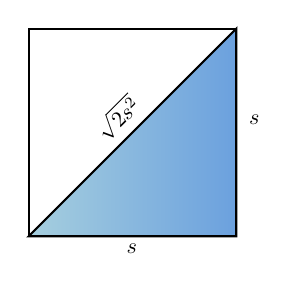
\begin{tikzpicture}[x=0.75pt,y=0.75pt,yscale=-1,xscale=1]
%uncomment if require: \path (0,300); %set diagram left start at 0, and has height of 300

%Shape: Square [id:dp7714270080777281] 
\draw   (11,11) -- (111,11) -- (111,111) -- (11,111) -- cycle ;
%Straight Lines [id:da32192438670599244] 
\draw    (11,111) -- (111,11) ;
%Shape: Right Triangle [id:dp44587122145691993] 
\path  [shading=_kd3za2b5b,_oobf9zdtu] (111,11) -- (11,111) -- (111,111) -- cycle ; % for fading 
 \draw   (111,11) -- (11,111) -- (111,111) -- cycle ; % for border 



% Text Node
\draw (58.6,58.6) node [anchor=south] [inner sep=0.75pt]  [rotate=-315,xscale=0.8,yscale=0.8]  {$\sqrt{2s^{2}}$};
% Text Node
\draw (57,113.4) node [anchor=north west][inner sep=0.75pt]  [xscale=0.8,yscale=0.8]  {$s$};
% Text Node
\draw (116,51.4) node [anchor=north west][inner sep=0.75pt]  [xscale=0.8,yscale=0.8]  {$s$};


\end{tikzpicture}
    \caption{A special case of the Pythagorean Theorem where each side is side length $s$ and the hypotenuse is $\sqrt{2s^2}$.}
    \label{fig:pythagSquare}
\end{figure}

\section{Distance between Points}

What is the distance between these two points?\index{distance using Pythagorean theorem}

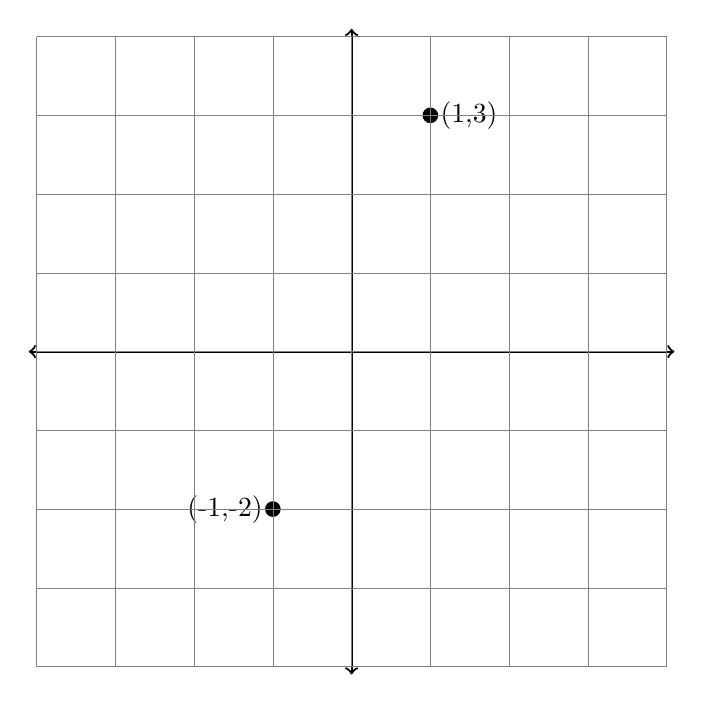
\begin{tikzpicture}
  % axis
  \draw[thick, <->] (0, -4.1) -- (0, 4.1);
  \draw[thick, <->] (-4.1, 0) -- (4.1, 0);
  \coordinate [circle, fill, inner sep=2pt] (a) at (-1,-2) ;
  \coordinate [circle, fill, inner sep=2pt] (b) at (1,3) ;
  \node [left] at (a) {(-1,-2)};
  \node [right] at (b) {(1,3)};
  % grid
  \draw[help lines, step = 1cm] (-4, -4) grid (4, 4);
  
\end{tikzpicture}

We can draw a right triangle and use the Pythagorean Theorem:

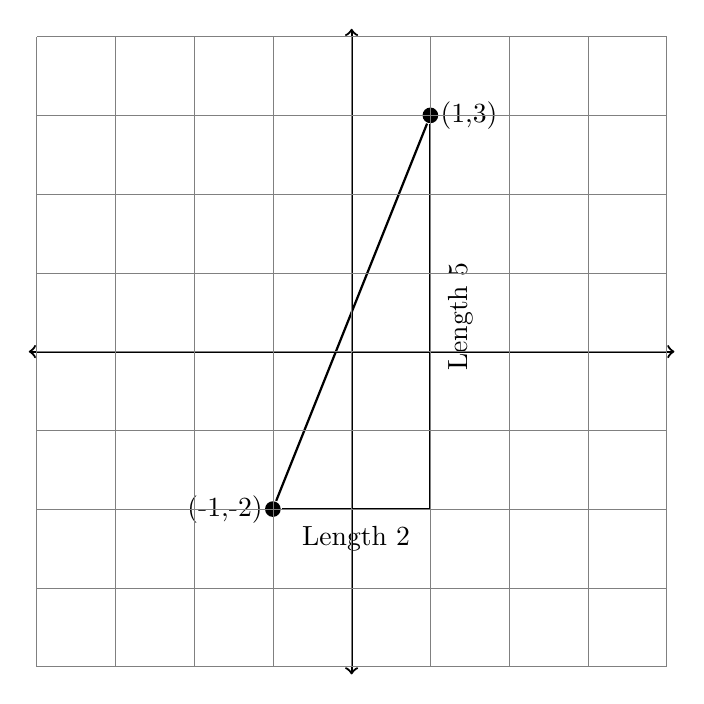
\begin{tikzpicture}
  % axis
  \draw[thick, <->] (0, -4.1) -- (0, 4.1);
  \draw[thick, <->] (-4.1, 0) -- (4.1, 0);
  \coordinate [circle, fill, inner sep=2pt] (a) at (-1,-2) ;
  \coordinate [circle, fill, inner sep=2pt] (b) at (1,3) ;
    \node [left] at (a) {(-1,-2)};
  \node [right] at (b) {(1,3)};
  \coordinate (c) at (1, -2);

  \draw [thick] (a) -- (b);
  \draw [thick] (a) -- node[outer sep = 3pt, below]{Length 2}(c);
  \draw [thick] (c) -- node[rotate=90, outer sep = 3pt, below]{Length 5}(b);
  \draw[help lines, step = 1cm] (-4, -4) grid (4, 4);
 
\end{tikzpicture}


The distance between the two points is $\sqrt{2^2 + 5^2} = \sqrt{29}
\approx 5.385165$. In other words, you square the change in $x$ and add it to
the square of the change in $y$. The distance is the square root of
that sum.

\section{Distance in 3 Dimensions}

What if the point is in three-dimensional space?  For example, you move 2
meters East, 8 meters North, and 4 meters up in the air. How far are
you from where you started?  You just square each, sum them, and take the square root:
$\sqrt{2^2 + 8^2 + 4^2} = \sqrt{84} = 2\sqrt{21} \approx 9.165$ meters.\index{distance!in 3 dimensions}

\begin{tikzpicture}
  \draw [thick, ->] (0,0,0) -- (9,0,0) node[outer sep = 1pt, right]{North} ; 
  \draw [thick, ->]  (0,0,0) -- (0,3,0) node[outer sep = 1pt, above]{Up} ; 
  \draw [thick, ->] (0,0,0) -- (0,0,4) node[outer sep = 1pt, below]{East} ; 

    \draw [dashed]  (8,0,0) -- node[outer sep = 1pt, right]{2}  (8,0,2); 

  \draw [dashed]  (0,0,2) -- node[outer sep = 1pt, below]{8} (8,0,2); 
  \draw [dashed]  (8,0,2) -- node[outer sep = 1pt, right]{4} (8,4,2); 
  \draw [thick]  (0,0,0) --  (8,4,2) node[circle, fill, inner sep=2pt]{}; 
  \node [left] at (5, 2.7, 1){$\sqrt{2^2 + 8^2 + 4^2} \approx 9.165$};

\end{tikzpicture}

This leads us to a formal definition of the distance formula:
\[
d = \sqrt{(x_2 - x_1)^2 + (y_2 - y_1)^2}
\]
Or in 3D space:
\[
d = \sqrt{(x_2 - x_1)^2 + (y_2 - y_1)^2 + (z_2 - z_1)^2}
\]
